\subsection{Homomorphic Predicate Evaluation}\label{block: comparison}
% ckks filtering method limitation
Since predicate evaluations are essentially concatenated comparisons,
the core computation here
is the comparison between two encrypted ciphertexts.
In this section,  we outline a series of homomorphic algorithms we devised
that lead to the proposed homomorphic comparison algorithm 
$\homcomp$, which supports unbounded-depth homomorphic predicate evaluation. % and then describe 
% \revise{how it supports 
% efficient and unbounded predicate evaluation.}

\subsubsection{The Main Building Block: $\hmsb$}
We first discuss the homomorphic most significant bit (MSB) extraction algorithm, $\hmsb$, 
which is the key building block in instantiating $\homcomp$.
We first point out that, as observed in the existing works~\cite{heda, pegasus,largeprecision}, 
the comparison between two ciphertexts $ct_a$ and $ct_b$ encrypting integers $a$ and $b$
can be evaluated by extracting the MSB from $ct_a-ct_b$,
% For instance, to evaluate $a \geq b$, we compute $a -b$ and homomorphically
% extract the MSB of the reduction result. 
since the MSB of the subtraction result encrypts a value of $0$ when $a \geq b$ and 
a value of $1$ when $a \textless b$. 
However, we observe that existing homomorphic MSB extraction algorithms following the $\pbs$ 
procedure~\cite{pegasus} proposed  in~\cite{DBLP:conf/asiacrypt/tfhepbs}
may not fit encrypted databases due to their low accuracy. In particular, such algorithms
can only successfully extract the MSB when the plaintext message (which is the
subtraction result $a-b$ here)
is an integer that is less than 6 bits (the full $\pbs$-based MSB extraction algorithm can be
found in the Appendix).
%We detail the algorithm in \cref{algo: kHMSB}.
% with 
% a MSB extraction function $\msb(x) = x \geq 0 ?$ $ 0 : 1$
% is limited to small precision (less than 6 bits). 
% The main obstacle is that the precision of PBS is strictly 
% related to the parameters of the test vector 
% as we mentioned in ...
% In order to obtain high precision, one adopts a test vector with a larger
% degree or represents a high-bit ciphertext with several low-bit ciphertexts, 
% which results in an increased computation cost or storage consumption.

% {\bf{Arbitrary Precision $\hmsb$}}: 
To overcome the precision loss problem while retaining high performance,
we propose a new homomorphic MSB extraction algorithm $\hmsb$.
% to overcome the above precision loss problem.
% To overcome this, we propose our innovative method to overcome
% the tussle between latency and precision
% In this section, we propose our novel homomorphic comparison algorithm
% \texttt{HomCom} where both the inputs are ciphertexts.
% {\bf{Key Technique}}: 
% convert a high-precision comparison to 
% a low-precision comparison by iterating PBS. 
The key idea of $\hmsb$ is to iterate the $\pbs$ algorithm
a certain number of times over the same ciphertext, such that we can
extract the MSB of arbitrary-precision messages. 
% and construct arbitrary precision homomorphic MSB extraction algorithm
% by iterating $\pbs$ and $k+1$-bit $\hmsb$.
% Then we utilize the arbitrary precision $\hmsb$ to implement 
% arbitrary precision homomorphic comparisons algorithm $\homcomp$.
% Our critical insight is that, in principle, the output of 
% homomorphic MSB extraction depends only on the first bit 
% of the plaintext, so we can homomorphically \textit{discard}
% the invalid bits and consider the result as low-precision 
% ciphertext with a larger scale. In \cref{algo: 2kHMSB}, we detail the exact 
% algorithm for constructing a $2k$-bit MSB extraction using
% $(k+1)$-bit MSB extractions and PBS.

%\subsubsection{Our solution via discarding invalid bit}



% {\bf{The Base Algorithm}}: We start with a standard homomorphic MSB extraction algorithm $\hmsb_{k+1}$ 
% by initializing a $\pbs$ operator with the MSB extraction function.
% % Pegasus~\cite{pegasus} and HEDA~\cite{heda} 
% to homomorphically extract the MSB of a $k+1$-bit ciphertext. 
% % In \cref{algo: kHMSB}, it can be seen that the standard 
% % MSB extraction algorithm basically follows the PBS procedure 
% % and the precision is limited due to the degree of the test vector.
% The $\hmsb_{k+1}$ operator basically follows the PBS procedure 
% and the precision is limited due to the degree of the test vector.
% We detail the exact algorithm in \cref{algo: kHMSB}.

\begin{algorithm}[t!]
    % \tiny
    \caption{$2k$-bit $\hmsb$}
    \label{algo: 2kHMSB}
    \SetKwInOut{Input}{Input}\SetKwInOut{Output}{Output}\SetKwInOut{Return}{Return}\SetKwComment{Comment}{$\triangleright$\ }{}
    \Input{A LWE ciphertext $ct_{I} = \lwe(m)$, where $m=2^{k}\cdot m_1 + m_0$.}
    \Input{A bootstrapping key $\bBK$.}
    \Output{A LWE ciphertext $ct_{O} = \lwe(\msb(m))$.}
    $ct_{1} \leftarrow 2^{k-1}ct_{I}$ 
    \Comment*[r]{$ct_{1} = \lwe(2^{2k-1}\lsb(m_1) + 2^{k-1}m_0)$} 
    $ct_{2} \leftarrow \hmsb_{k+1}(ct_{1}) $ 
    \Comment*[r]{$ct_{2} = \lwe(2^{2k-1}\lsb(m_{1}))$} 
    $ct_{3} \leftarrow ct_{1} - ct_{2}$ 
    \Comment*[r]{$ct_{3} = \lwe(2^{k-1}m_0)$} 
    $ct_{4} \leftarrow \pbs(ct_{3}, \bBK, T(x) = \frac{x}{2^{k-1}})$ 
    \Comment*[r]{$ct_{4} = \lwe(m_0)$} 
    $ct_{5} \leftarrow ct_{I} - ct_{4}$ 
    \Comment*[r]{$ct_{5} = \lwe(2^{k}m_1)$} 
    $ct_{O} \leftarrow \hmsb_{k}(ct_{5})$
    \Comment*[r]{$ct_{O} = \lwe(\msb(m))$} 
    \Return{$ct_{O} = \lwe(\msb(m))$}
\end{algorithm}

\begin{figure}[t!]
   \begin{center}
   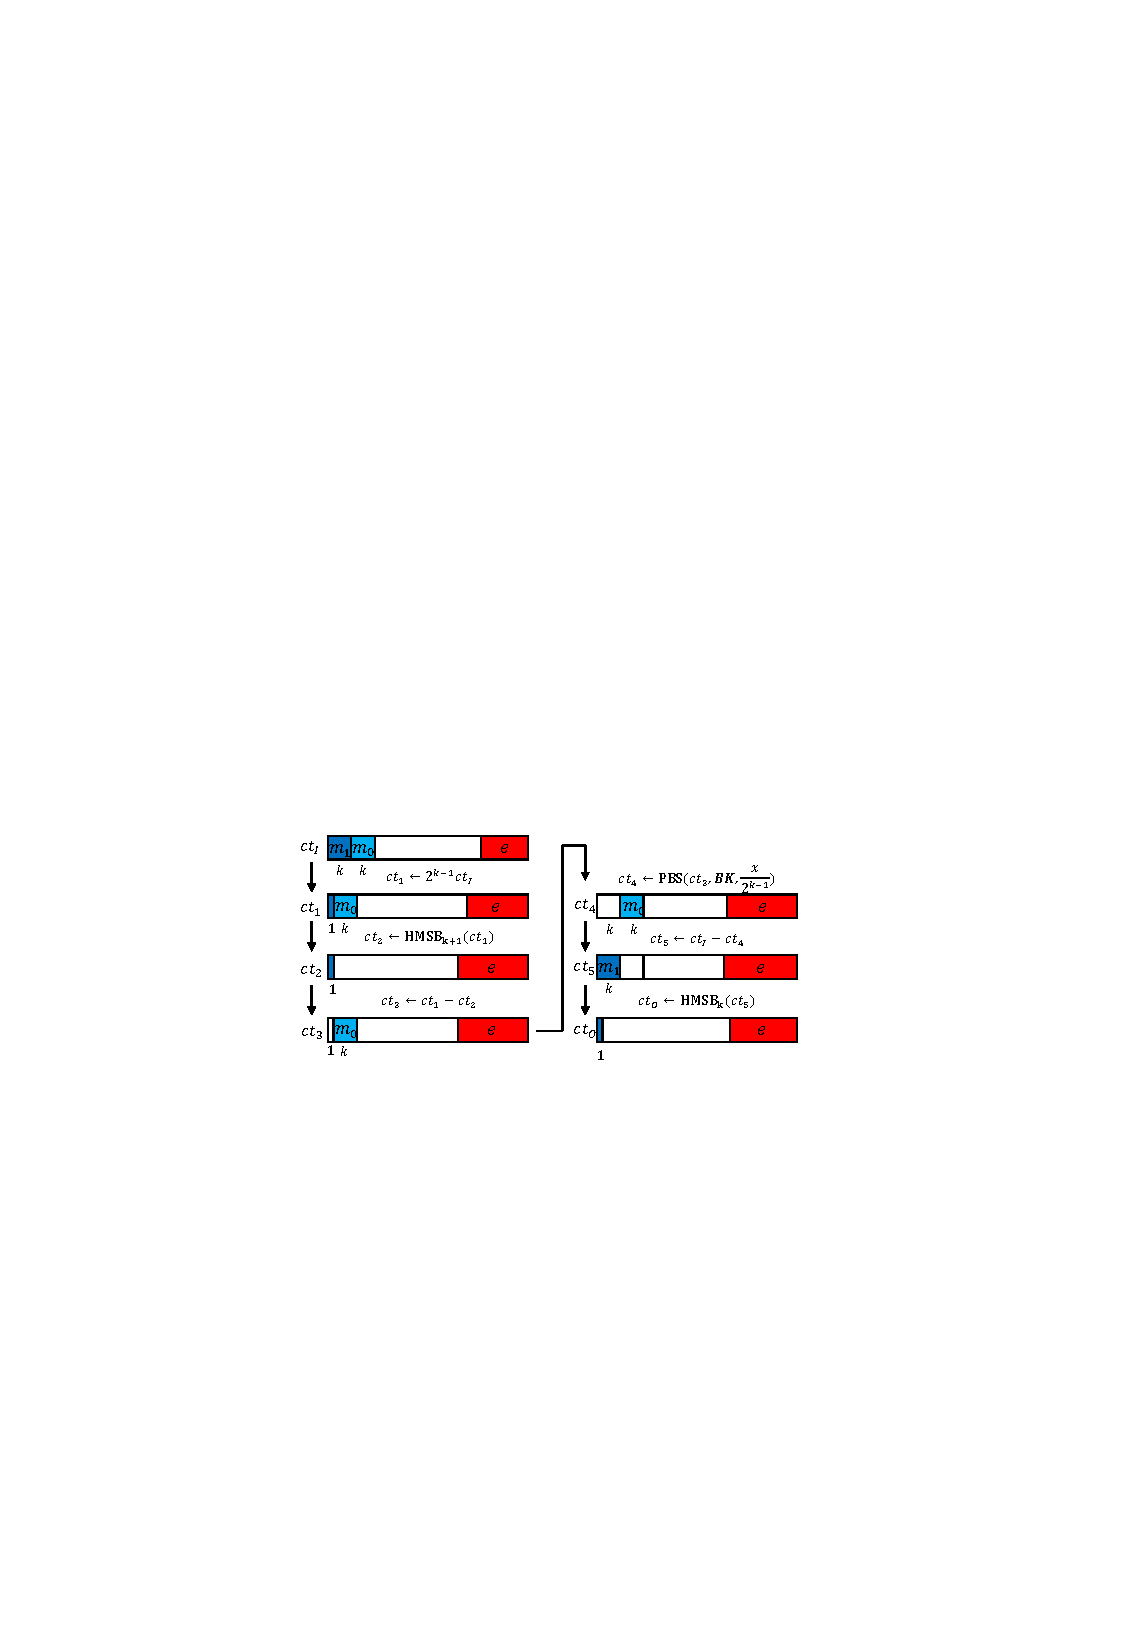
\includegraphics[width=\linewidth]{figure/hmsb.pdf}
   \end{center}
    % \vspace{-0.5em}
      \caption{A line-by-line illustration
      of how \cref{algo: 2kHMSB} works 
      with the input ciphertext $ct_{I}=\rlwe(2^{k}m_1+m_0)$.} 
      \Description{Figure 3. Fully described in the Algorithm 1}
   \label{fig: comparison}
   % \vspace{-0.5em}
\end{figure}

\begin{algorithm}[t!]
    % \tiny
    \caption{$tk$-bit $\hmsb$}
    \label{algo: tkHMSB}
    \SetKwInOut{Input}{Input}\SetKwInOut{Output}{Output}\SetKwInOut{Return}{Return}\SetKwComment{Comment}{$\triangleright$\ }{}
    \Input{A LWE ciphertext $ct_{I} = \lwe(m)$, where 
    $m=\sum_{i = 0}^{t}2^{ik} \cdot m_{i}$.}
    \Input{A bootstrapping key $\bBK$.}
    \Output{A LWE ciphertext $ct_{O} = \lwe(\msb(m))$.}
    \eIf{$t == 1$}
    {
        $ct_{O} \leftarrow \hmsb_{k}(ct_{I})$ \\
    }
    {
        $ct_{1} \leftarrow 2^{tk-1}ct_{I}$ \\
        % \Comment*[r]{$ct_{1} = {\rm LWE}(2^{(t+1)k-1}{\rm LSB}(m_1) + 2^{tk-1}m_0)$} \\
        $ct_{2} \leftarrow \hmsb_{k+1}(ct_{1}) $ \\
        % \Comment*[r]{$ct_{2} = {\rm LWE}(2^{(t+1)k-1}{\rm LSB}(m_{1}))$} \\
        $ct_{3} \leftarrow ct_{1} - ct_{2}$ \\
        % \Comment*[r]{$ct_{3} = {\rm LWE}(2^{tk-1}m_0)$} \\
        $ct_{4} \leftarrow \pbs(ct_{3}, \bBK, T(x) = \frac{x}{2^{tk-1}})$  \\
        % \Comment*[r]{$ct_{4} = {\rm LWE}(m_0)$} \\
        $ct_{5} \leftarrow ct_{I} - ct_{4}$  \\
        % \Comment*[r]{$ct_{5} = {\rm LWE}(m-m_{0})$} \\
        $ct_{O} \leftarrow \hmsb_{tk}(ct_{5})$ \\
        % \Comment*[r]{$ct_{O} = {\rm LWE}({\rm MSB}(m))$} \\
    }
    \Return{$ct_{O} = \lwe(\msb(m))$}
\end{algorithm}

We start with a $\pbs$-based MSB extraction algorithm, named $\pbshmsb$. 
We assume that $\pbshmsb$ can successfully extract the MSB of a $\kappa$-bit integer 
(e.g., as mentioned, $\kappa=6$ using the original $\pbs$ method
proposed in~\cite{DBLP:conf/asiacrypt/tfhepbs}).
Let $k=\kappa-1$ (e.g., $k=5$ in our implementation), 
we show how to construct a $2k$-bit homomorphic
MSB extraction algorithm based on $\pbshmsb$ in \cref{algo: 2kHMSB}.
First, given a $2k$-bit input ciphertext 
$ct_{I} = \lwe(m)$, it is obvious that $m=2^{k}\cdot m_1 + m_0$. 
Our critical insight is that the MSB
of $ct_{I}$ depends only on the first bit 
of the plaintext, so we can homomorphically remove
the remaining bits to construct a $k$-bit ciphertext.
% the invalid bits and consider the result as low-precision 
% ciphertext with a larger scale.
To achieve the bit removal, as depicted in \cref{fig: comparison},
we homomorphically shift the internal
plaintext message towards the left, which turns $\lwe(2^k \cdot m_1+m_0)$ 
into $\lwe(m_0)$. Next, we can homomorphically
subtract $\lwe(m_0)$ from $\lwe(m)=\lwe(2^k\cdot m_1+m_0)$, and get $\lwe(2^k\cdot m_1)$.
%to get a $k$-bit ciphertext $\lwe(2^k \cdot m_1)$.
Then, we can simply apply $\pbshmsb$ to extract the MSB of the $k$-bit plaintext message 
$m_1$, which is also the MSB of $\lwe(m)$, i.e., $ct_{I}$.
%However, to correctly
%bootstrap a ciphertext~\cite{pegasus, DBLP:conf/asiacrypt/tfhepbs}, 
%the MSB of the encrypted plaintext needs to be set to zero.
%To address this problem, we should keep one bit in the shifting processing 
%and zero it.

Based on a similar idea, we can extend the $2k$-bit
$\hmsb$ to arbitrary precision $tk$ for any positive integer $t$ by repeatedly 
shifting and subtracting $k$-bit plaintext messages. As formalized in \cref{algo: tkHMSB},
we first recursively discard the least significant $k$ bits of the initial $tk$-bit ciphertext
$t$ times until only the most significant $k$ bits remain. Then, we simply apply 
$\pbshmsb$ with $\kappa$-bit precision and accurately extract the MSB of the input
ciphertext with $tk$-bit-precision plaintext message.
%existing low-precision homomorphically MSB extraction methods~\cite{pegasus, heda}.

% By applying ${\rm HMSB}_{k+1}$ to $ct_{1}$, we get 
% $ct_{2} = {\rm LWE}_{n,q}(2^{2k-1}{\rm LSB}(m_{1}))$, which
% encrypts the LSB of $m_{1}$. 
% Then, we substract $ct_{2}$ from $ct_{1}$ and get $ct_{3}$ where 
% $ct_{3}$ which encrypts $2^{k-1}m_{0}$. After steps 2 and 3, we 
% have discarded the MSB of the encrypted plaintext and we can apply 
% PBS to $ct_{3}$. 
% and get $ct_{1}$
% . After the shifting process, 
% the most $(k-1)$bits of $m_{1}$ have been 
% moved as shown in \cref{fig: comparison}. 
% However, to correctly
% bootstrap a ciphertext, the MSB of the encrypted plaintext needs to be set to zero.
% To address this problem, we should remove the MSB of plaintext.
% By applying ${\rm HMSB}_{k+1}$ to $ct_{1}$, we get 
% $ct_{2} = {\rm LWE}_{n,q}(2^{2k-1}{\rm LSB}(m_{1}))$, which
% encrypts the LSB of $m_{1}$. 
% Then, we substract $ct_{2}$ from $ct_{1}$ and get $ct_{3}$ where 
% $ct_{3}$ which encrypts $2^{k-1}m_{0}$. After steps 2 and 3, we 
% have discarded the MSB of the encrypted plaintext and we can apply 
% PBS to $ct_{3}$. By applying PBS to $ct_{3}$, we get $ct_{4} = {\rm LWE}_{n,q}(m_0)$. And then, computing $ct_{I} - ct_{4}$, we get 
% $ct_{5} = {\rm LWE}_{n,q}(2^{k}m_1)$. Until now we have removed the 
% least $k$ bits of $m$. Finally, by applying ${\rm HMSB}_{k}$ 
% to $ct_{5}$, we obtain $ct_{O} = {\rm LWE}_{n,q}({\rm MSB}(m))$.

% \begin{algorithm}[t!]
%     % \tiny
%     \caption{$k$-bit \texttt{HMSB}}
%     \label{algo: kHMSB}
%     \SetKwInOut{Input}{Input}\SetKwInOut{Output}{Output}\SetKwInOut{Return}{Return}
%     \Input{A LWE ciphertext $ct_{I} = {\rm LWE}^{n,q}_{\mathbf{s}}(m) 
%     = (b, \mathbf{a})$, where $m \ in [0, 2^{k} -1]$.}
%     \Input{A constant $\mu = q / 4$.}
%     \Input{A bootstrapping key $\mathbf{BK}$, where 
%     $\mathbf{BK}\left[i\right] = \reg{RGSW}^{N,q}_{\Tilde{s}}(\mathbf{s}[i])$, for $i \in [1,n]$}
%     \Output{A LWE ciphertext $ct_{O} = {\rm LWE}_{\mathbf{s}}^{n,q}({\rm MSB}(m))$.}
%     % $b \leftarrow \lfloor \frac{2N}{q}b \rceil$ 
%     % and $\mathbf{a} \leftarrow \lfloor \frac{2N}{q}\mathbf{a} \rceil$ \\
%     $\Tilde{v} \leftarrow \mu \cdot (1 + x^2 + x^3 + ... + x^{N-1}) $ \\
%     $ACC \leftarrow \texttt{BlindRotate}(\Tilde{v}, ct_I, \mathbf{BK})$ \\
%     $ct_{O} = (b', \mathbf{a'}) = \texttt{SampleExtract}(ACC)[0]$ \\
%     \Return{$ct_{O} = (b' + \mu, \mathbf{a}) 
%     = {\rm LWE}_{\mathbf{s}}^{n,q}({\rm MSB}(m))$}
% \end{algorithm}



% \begin{figure*}[t!]
%    \begin{center}
%    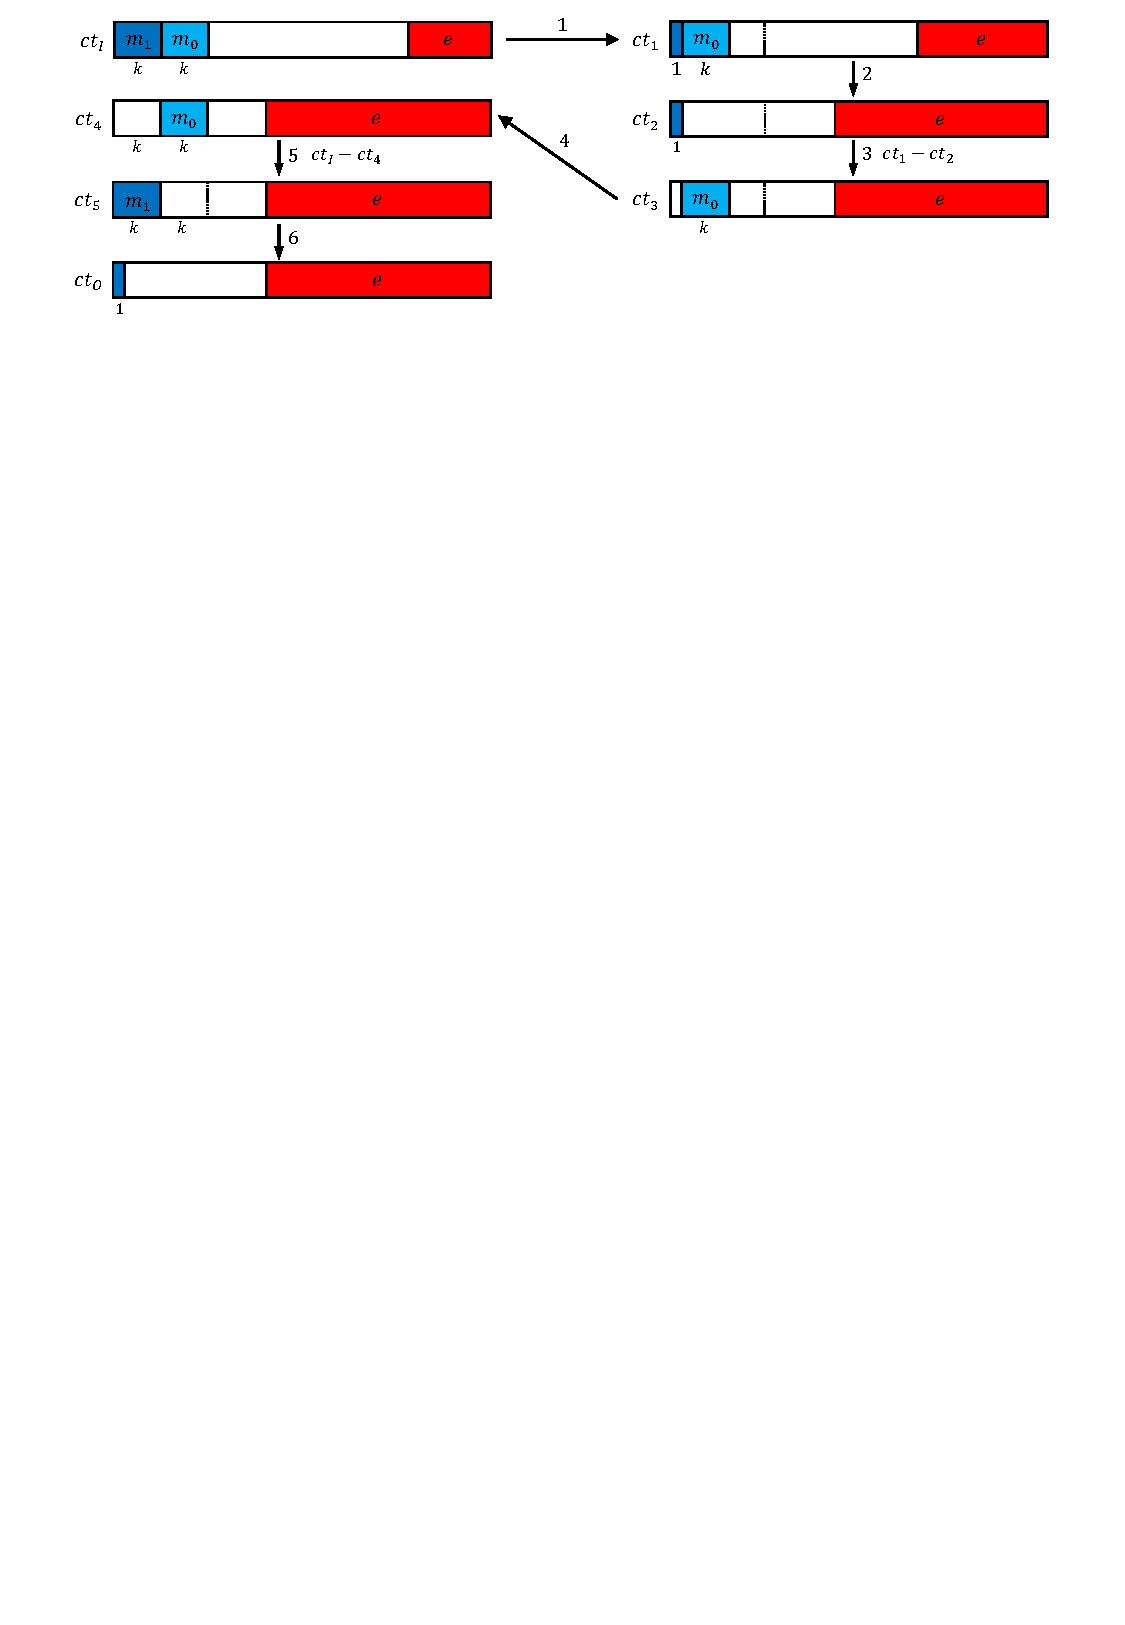
\includegraphics[width=0.75\linewidth]{figure/comparison.pdf}
%    \end{center}
%     \vspace{-0.5em}
%       \caption{A plaintext illustration in \cref{algo: 2kHMSB}. 
%       Each rectangle represents a decrypted plaintext while the left is 
%       the most significant bit.
%       The blue-colored region is the bits occupied by the message, 
%       the red-colored field is the bits filled with noise, 
%       and the white part is the bits set to zero.} 
%    \label{fig: comparison}
%    \vspace{-0.5em}
% \end{figure*}



%\subsubsection{Generality algorithm}
%\subsubsection{High-Precision Recursive HMSB}


% {\bf{Arbitrary Precision HMSB}}: 
% Given an input ciphertext $ct_{I} = {\rm LWE}_{n,q}(m)$, 
% where $m=\sum_{i = 0}^{t}2^{ik} \cdot m_{i}$.
% As shown in \cref{algo: tkHMSB}, in generality, we shift the ciphertext
% $(tk-1)$bits to move the most $(tk-1)$bits of $m$ 
% and reserve the least $(k+1)$bits. 
% The goal of the next four steps (line 2-5) is to move $m_{0}$ from $m$ 
% in an encrypted form, which is the same as \cref{algo: 2kHMSB}. 
% After that, we get the ciphertext $ct_{5}={\rm LWE}_{n,q}(m-m_0)$ and the 
% $m-m_{0}$ can be regarded as a $tk$-bit precision plaintext.
% By adopting ${\rm HMSB}_{tk}$ to $ct_{5}$, we obtain $ct_{O}$
% that encrypts the MSB of $m$.

\begin{algorithm}[t!]
    % \tiny
    \caption{$\homcomp$}
    \label{algo: homcom}
    \SetKwInOut{Input}{Input}\SetKwInOut{Output}{Output}\SetKwInOut{Return}{Return}\SetKwComment{Comment}{$\triangleright$\ }{}
    \Input{Two ciphertexts $ct_{a} = \lwe(a), ct_{b} = \lwe(b)$.}
    \Input{Comparison operator $\cmp$.}
    \Input{A bootstrapping key $\bBK$.}
    \Output{A LWE ciphertext $ct_{O} = \lwe(c)$
    where $c = 1$ if $a$ $\cmp$ $b$ is True, else $c = 0$.}
    \Switch{$\cmp$}
    {
        \lCase{$\geq$}{$ct_O \leftarrow \homgate((\hmsb(c_a-c_b), \reg{NOT}))$} \\
        \lCase{$>$}{$ct_O \leftarrow \hmsb(c_b-c_a)$} \\
        \lCase{$\leq$}{$ct_O \leftarrow \homgate(\hmsb(c_b-c_a), \reg{NOT})$} \\
        \lCase{$<$}{$ct_O \leftarrow \hmsb(c_a-c_b)$} \\
        \uCase{$==$}
        {
            $ct_O \leftarrow \homgate(\hmsb(c_a - c_b),\hmsb(c_b - c_a), \reg{NOR})$ \\
        }
        \uCase{$\ne$}
        {
            $ct_O \leftarrow \homgate(\homcomp(ct_a, ct_b, ==), \reg{NOT})$ \\
        }
    }
    % \uIf{$\cmp$ is $\geq$}
    % {
    %     $ct_O \leftarrow \homgate((\hmsb(c_a-c_b), \reg{NOT}))$ \\
    % }
    % \uElseIf{$\cmp$ is $>$}
    % {
    %     $ct_O \leftarrow \hmsb(c_b-c_a)$ \\
    % }
    % \uElseIf{$\cmp$ is $\leq$}
    % {
    %     $ct_O \leftarrow \homgate(\hmsb(c_b-c_a), \reg{NOT})$ \\
    % }
    % \uElseIf{$\cmp$ is $<$}
    % {
    %     $ct_O \leftarrow \hmsb(c_a-c_b)$ \\
    % }
    % \uElseIf{$\cmp$ is $==$}
    % {
    %     $ct_O \leftarrow \homgate(\hmsb(c_a - c_b),
    %      \hmsb(c_b - c_a), \reg{NOR})$ \\
    % }
    % \uElse
    % {
    %     $ct_O \leftarrow \homgate(\hmsb(c_a - c_b),
    %      \hmsb(c_b - c_a), \reg{NAND})$ \\
    % }
    \Return{$ct_{O} = {\rm LWE}(c)$}
\end{algorithm}
%\subsubsection{Homomorphic Comparison in EDBMS}
\subsubsection{$\homcomp$ Based on $\hmsb$}
Based on the arbitrary-precision $\hmsb$ algorithm devised above, we can carry
out arbitrary-precision comparisons between the queried attributes and the DB items.
Let $ct_a$ and $ct_b$ be the two LWE ciphertexts
that encrypt $a$ and $b$, and
$\cmp$ be the type of comparison to be performed ($\geq, >, \leq, <, ==, \ne$).
$\homcomp(ct_a, ct_b, \cmp)$ 
outputs an LWE ciphertext encrypting $1$
if the predicate $a$ $\cmp$ $b$ is true 
and $0$ if $a$ $\cmp$ $b$ is false.
The $\homcomp$ algorithm
can be easily constructed using $\hmsb$
with some additional homomorphic gates.
We summarize the exact arithmetic procedure for
$\homcomp$ in \cref{algo: homcom}. The complexity of our
$\homcomp$ algorithm can be expressed by the following lemma,
where the formal proof is given in the Appendix.

\begin{lemma}
    Given the two $tk$-bit ciphertext $ct_a$, $ct_b$ with
    a comparison operator $\homcomp$, the \cref{algo: homcom}
    outputs LWE ciphertext $ct_{O} = \lwe(c)$
    where $c = 1$ if $a$ $\cmp$ $b$ is True, else $c = 0$.
    The number of $\pbs$ evaluated by \cref{algo: homcom} 
    is $2t-1$ or $2t$.
    \label{lemma: homcomp}
\end{lemma}



% \begin{table}[htbp] 
%     \centering
%     \caption{Constructing \texttt{HomCom} using \texttt{HMSB}}
%     \vspace{-0.5em}
%         \begin{tabular}{cc}
%             \toprule
%             Comparison Type & Homomorphic Operation \\%\texttt{HomCom} & Operation \\
%             \midrule
%             $\texttt{HomComp}(c_1, c_2, \geq)$ & 
%             $\texttt{NOT}(\texttt{HMSB}(c1-c2))$\\
%             $\texttt{HomComp}(c_1, c_2, >)$ & 
%             $\texttt{HMSB}(c2-c1)$ \\
%             $\texttt{HomComp}(c_1, c_2, \leq)$ & 
%             $\texttt{NOT}(\texttt{HMSB}(c2-c1))$\\
%             $\texttt{HomComp}(c_1, c_2, <)$ & 
%             $\texttt{HMSB}(c1-c2)$ \\
%             $\texttt{HomComp}(c_1, c_2, ==)$ & 
%             $\texttt{HomComp}(c_1, c_2, \geq)$  
%             \texttt{AND} $\texttt{HomCom}(c_1, c_2, \leq)$ \\
            
            
%             \bottomrule
%         \end{tabular}
%     \label{tab:homcom}
% \end{table}



